\section{DSIR：importance resampling}

\subsection{重要性采样复习}

DSIR 的关键直觉来自重要性采样。假设你想从目标分布 $p$ 采样，但你只能从 proposal 分布 $q$ 采样，那么你先从 $q$ 抽样，再用权重
\[
w(x)\propto \frac{p(x)}{q(x)}
\]
重新加权，最后再按权重重采样。这样得到的样本集合会更接近 $p$。

\begin{figure}[H]
\centering
\begin{tikzpicture}[every node/.style={font=\small, align=center}]
\node[draw, rounded corners, fill=orange!12, minimum width=2.9cm, minimum height=0.9cm] (q) at (0,0) {proposal $q$\\easy to sample};
\node[draw, rounded corners, fill=yellow!16, minimum width=3.0cm, minimum height=0.9cm] (w) at (4.4,0) {weights $p/q$\\reweight};
\node[draw, rounded corners, fill=green!14, minimum width=3.1cm, minimum height=0.9cm] (p) at (8.9,0) {resample $p$\\desired distribution};
\draw[-{Latex[length=3mm]}, thick] (q) -- (w);
\draw[-{Latex[length=3mm]}, thick] (w) -- (p);
\end{tikzpicture}
\caption{importance resampling 的基本三步：先采样，再重权重，最后重采样}
\end{figure}

\begin{importantbox}{DSIR 的价值}
和只做二分类相比，显式估计 $p/q$ 更接近“我到底想要什么数据”的原始目标。它会更自然地兼顾多样性与覆盖性，而不仅仅是挑出最像的那批。
\end{importantbox}

\subsection{为什么重要性采样是对的}

如果你关心的不是单个样本，而是某个函数 $f(x)$ 在目标分布下的期望，那么重要性采样给出的是
\[
\mathbb{E}_{p}[f(x)] = \frac{\mathbb{E}_{q}[w(x)f(x)]}{\mathbb{E}_{q}[w(x)]}.
\]
这条式子说明：只要权重 $w(x)$ 估得够好，你就可以从 proposal 分布的样本上，近似恢复目标分布的统计量。

\begin{knowledgebox}{这和过滤的关系}
过滤不是必须严格“采样到目标分布”，但如果你能让保留的数据在统计上更接近目标分布，那么后续训练通常会更稳。DSIR 的价值就在于它把“像不像”升级成了“分布像不像”。
\end{knowledgebox}

\subsection{从分布到文档}

真正的数据选择不是在理想分布上抽象地采样，而是在小目标数据集 $D_p$ 和大原始数据集 $D_q$ 上落地。DSIR 的难点也在这里：$D_p$ 太小，没法直接训练复杂分布模型。所以课程里给出的办法是把文本先做 hash n-gram，再估计低维分布。

\begin{figure}[H]
\centering
\begin{tikzpicture}[node distance=1.3cm, every node/.style={font=\small, align=center}]
\node[draw, rounded corners, fill=green!10, minimum width=3.0cm, minimum height=0.85cm] (dp) {small target set $D_p$};
\node[draw, rounded corners, fill=orange!12, right=of dp, minimum width=3.0cm, minimum height=0.85cm] (dq) {large raw set $D_q$};
\node[draw, rounded corners, fill=yellow!16, below=of dq, minimum width=3.4cm, minimum height=0.85cm] (hash) {hash n-grams};
\node[draw, rounded corners, fill=blue!14, below=of hash, minimum width=3.4cm, minimum height=0.85cm] (res) {estimate weights / resample};
\draw[-{Latex[length=3mm]}, thick] (dp) -- (hash);
\draw[-{Latex[length=3mm]}, thick] (dq) -- (hash);
\draw[-{Latex[length=3mm]}, thick] (hash) -- (res);
\end{tikzpicture}
\caption{DSIR 的工程落点：把难以建模的文本分布，压缩到 hash n-gram 空间里估权重}
\end{figure}

\begin{warningbox}{DSIR 不是银弹}
它仍然依赖简化表示。如果 hash n-gram 太粗，权重就会失真；如果特征太细，目标数据又会不够支撑估计。它只是把“更原则化”的问题变成一个更可控的近似。
\end{warningbox}

\subsection{为什么它有时优于 heuristic classifier}

fastText 的做法很像“判定这个样本像不像目标类”，而 DSIR 更像“让样本集整体更接近目标分布”。后者在多样性和覆盖性上通常更自然，也更适合用于构造更均衡的数据子集。

\begin{figure}[H]
\centering
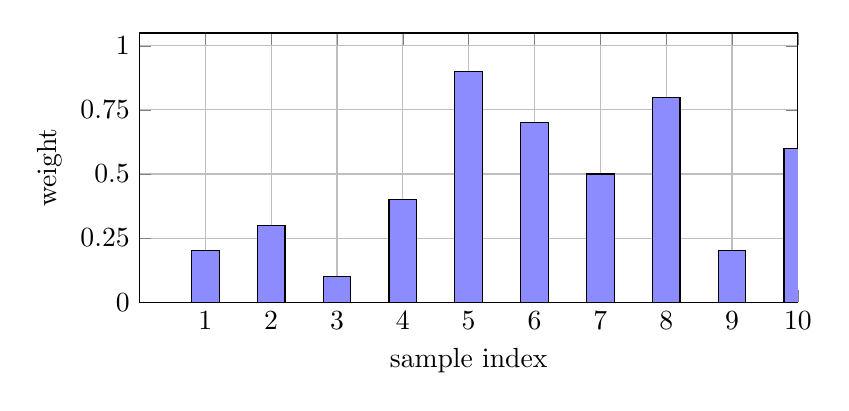
\begin{tikzpicture}
\begin{axis}[
    width=0.82\textwidth,
    height=5cm,
    xlabel={sample index},
    ylabel={weight},
    ymin=0, ymax=1.05,
    xmin=0, xmax=10,
    xtick={1,2,3,4,5,6,7,8,9,10},
    ytick={0,0.25,0.5,0.75,1.0},
    grid=both,
]
\addplot[ybar, fill=blue!45] coordinates {(1,0.2) (2,0.3) (3,0.1) (4,0.4) (5,0.9) (6,0.7) (7,0.5) (8,0.8) (9,0.2) (10,0.6)};
\end{axis}
\end{tikzpicture}
\caption{importance weight 的直观含义：proposal 里抽到的样本并不均匀，需要按权重修正}
\end{figure}

\subsection{实现时要小心什么}

实做 DSIR 时，最容易出问题的是权重极端不均匀。少数样本权重特别大，会导致重采样几乎只剩它们，结果失去多样性。常见做法包括权重截断、归一化、平滑和分桶。

\begin{table}[H]
\centering
\small
\renewcommand{\arraystretch}{1.15}
\begin{tabular}{p{3.0cm}p{4.2cm}p{4.2cm}}
\toprule
\textbf{问题} & \textbf{现象} & \textbf{常见处理} \\
\midrule
权重过尖 & 少数样本统治结果 & clipping / smoothing \\
特征过稀 & 估计方差很大 & 降维 / hash / 合并桶 \\
目标集太小 & 权重不稳定 & 先做粗过滤再 DSIR \\
\bottomrule
\end{tabular}
\caption{DSIR 的几个典型失败模式和应对方式}
\end{table}

\subsection{和 heuristic filter 的取舍}

如果你只想快速删掉一大批明显不相关的网页，heuristic classifier 往往够了。但如果你要认真控制保留下来的数据分布，比如想让某个主题、体裁或领域的比例更合理，DSIR 通常更符合目标。

